% ---------------------------------------------------------------------
% 2.5 El paradigma P300 Speller
% ---------------------------------------------------------------------
\section[EL PARADIGMA P300 SPELLER]{El paradigma P300 Speller}
\label{sec:speller}

\subsection{Deletreador de Farwell y Donchin}

En 1988 Farwell y Donchin publicaron el sistema que hoy se conoce como P300 Speller o deletreador
de Donchin. En su artículo original todavía no se habla de una BCI, sino de una prótesis mental
pensada como canal de comunicación para personas cuya discapacidad motora les impide comunicarse
\cite{farwell1988}. El sistema muestra en pantalla una matriz de $6\times6$
celdas con las letras del alfabeto, algunos números y comandos simples. Durante su funcionamiento,
las filas y columnas se iluminan una por una en orden aleatorio. Mientras tanto, el usuario se
concentra en la celda que desea seleccionar, por ejemplo, contando mentalmente cuántas veces se
ilumina \cite{farwell1988}. De los doce eventos posibles, seis
filas y seis columnas, solo dos contienen al carácter objetivo. Esas dos intensificaciones hacen el
papel de los estímulos raros del paradigma \textit{oddball} y provocan una P300 que no aparece en
las otras diez, como se representa en la Figura~\ref{fig:matriz}.

\begin{figure}[htbp]
\centering
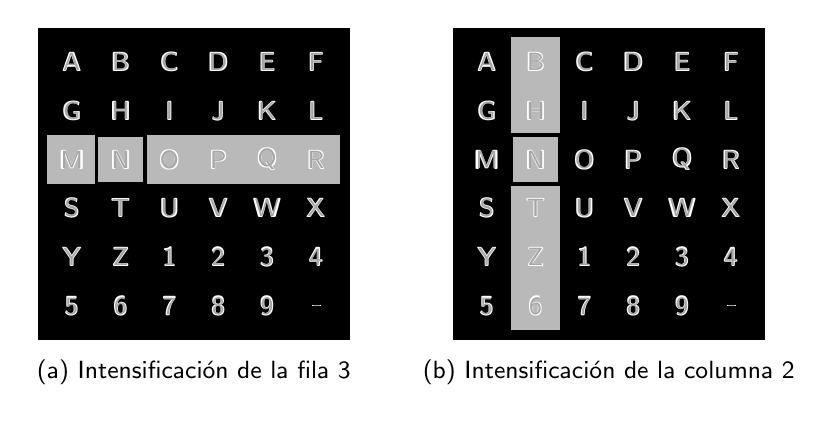
\begin{tikzpicture}[scale=0.62, every node/.style={font=\sffamily\small}]
  \def\letras{{"A","B","C","D","E","F","G","H","I","J","K","L","M","N","O","P","Q","R",
               "S","T","U","V","W","X","Y","Z","1","2","3","4","5","6","7","8","9","\_"}}
  % matriz izquierda: fila 3 intensificada
  \begin{scope}
    \fill[black] (-0.2,-0.2) rectangle (6.2,6.2);
    \fill[gray!55] (0,3) rectangle (6,4);
    \foreach \i in {0,...,35}{
      \pgfmathtruncatemacro{\f}{int(\i/6)}
      \pgfmathtruncatemacro{\c}{mod(\i,6)}
      \pgfmathsetmacro{\l}{\letras[\i]}
      \ifthenelse{\f=2}
        {\node[text=white, font=\sffamily\bfseries] at (\c+0.5,5.5-\f) {\l};}
        {\node[text=gray!70] at (\c+0.5,5.5-\f) {\l};}
    }
    \draw[black, very thick] (1,3) rectangle (2,4);
    \node[below, align=center] at (3,-0.4) {(a) Intensificación de la fila 3};
  \end{scope}
  % matriz derecha: columna 2 intensificada
  \begin{scope}[xshift=8.5cm]
    \fill[black] (-0.2,-0.2) rectangle (6.2,6.2);
    \fill[gray!55] (1,0) rectangle (2,6);
    \foreach \i in {0,...,35}{
      \pgfmathtruncatemacro{\f}{int(\i/6)}
      \pgfmathtruncatemacro{\c}{mod(\i,6)}
      \pgfmathsetmacro{\l}{\letras[\i]}
      \ifthenelse{\c=1}
        {\node[text=white, font=\sffamily\bfseries] at (\c+0.5,5.5-\f) {\l};}
        {\node[text=gray!70] at (\c+0.5,5.5-\f) {\l};}
    }
    \draw[black, very thick] (1,3) rectangle (2,4);
    \node[below, align=center] at (3,-0.4) {(b) Intensificación de la columna 2};
  \end{scope}
\end{tikzpicture}
\caption{Matriz de $6\times6$ caracteres del P300 Speller. Si el usuario atiende a la letra N
(recuadro), tanto la intensificación de la fila 3 como la de la columna 2 son eventos objetivo que
provocan una P300. Las diez intensificaciones restantes son eventos no objetivo. Elaboración propia
con base en \cite{farwell1988}.}
\label{fig:matriz}
\end{figure}

El sistema original registraba el EEG únicamente en el electrodo Pz y, con cuatro participantes
sanos, alcanzó una exactitud cercana al 95\% con un tiempo promedio de 26 segundos por carácter,
equivalente a 2.3 caracteres o 12 bits por minuto \cite{farwell1988}. Aunque esta velocidad es muy
baja comparada con la escritura convencional, la arquitectura y el principio de operación de este
deletreador siguen siendo la base de la mayoría de los sistemas BCI basados en la P300
\cite{contreras2021}.

\subsection{Parámetros de estimulación}

El desempeño del P300 Speller depende en buena medida de los tiempos con que se presentan los
estímulos. La duración de la intensificación es el tiempo que una fila o columna permanece
iluminada. El intervalo entre estímulos (ISI) es el tiempo que la matriz permanece sin iluminar
antes del siguiente evento. La suma de ambos se conoce como intervalo entre inicios de estímulos
(SOA). A una secuencia completa de las doce intensificaciones se le llama repetición, y el número
de repeticiones que se hacen antes de elegir el carácter determina el equilibrio entre velocidad y
exactitud \cite{krusienski2008}. En la base de datos II de la tercera competencia BCI, utilizada
en la fase exploratoria de este trabajo, cada intensificación dura 100~ms seguida de 75~ms sin
estímulo, por lo que cada repetición dura alrededor de 2.1~s, y cada carácter se deletrea con 15
repeticiones, es decir, con 180 intensificaciones \cite{blankertz2006}.

\subsection{Épocas de EEG y decodificación del carácter}

Para clasificar la señal, el registro continuo se divide en segmentos que inician en el instante
de cada intensificación, llamados épocas. Una época es atendida si corresponde a una fila o
columna que contiene el carácter objetivo, y no atendida en caso contrario \cite{contreras2021}. En
lo sucesivo, $x^{f}_{j}$ y $x^{c}_{j}$ denotan las épocas asociadas a la fila $f$ y a la columna $c$
en la repetición $j$.

Una vez que un clasificador asigna a cada época un puntaje $g(\cdot)$ que refleja la probabilidad
de que contenga una P300, el carácter se decide sumando los puntajes de cada fila y cada columna a
lo largo de las $J$ repeticiones y eligiendo aquellas con el valor más alto \cite{rakotomamonjy2008}:
\begin{equation}
\hat{f} = \arg\max_{f\in\{1,\dots,6\}} \sum_{j=1}^{J} g\!\left(x^{f}_{j}\right), \qquad
\hat{c} = \arg\max_{c\in\{1,\dots,6\}} \sum_{j=1}^{J} g\!\left(x^{c}_{j}\right),
\label{eq:decodificacion}
\end{equation}
y el carácter seleccionado es el que está en la intersección de la fila $\hat{f}$ y la
columna $\hat{c}$. Con esta estrategia, el ganador de la competencia BCI III
alcanzó una exactitud del 96.5\% al utilizar las 15 repeticiones disponibles
\cite{rakotomamonjy2008}.

Por la propia estructura del paradigma, el conjunto de épocas está fuertemente
desbalanceado: en cada repetición solo dos de las doce intensificaciones son objetivo, lo que
produce una proporción de una época positiva por cada cinco negativas \cite{cecotti2011}. Si este
desbalance no se considera durante el entrenamiento, un clasificador puede alcanzar una exactitud
aparente cercana al 83\% simplemente prediciendo siempre la clase negativa, razón por la cual las
métricas de evaluación de la Sección~\ref{sec:metricas} deben elegirse con cuidado.

\subsection{Bases de datos públicas}

Gran parte de la investigación sobre detección de la P300 se apoya en bases de datos públicas, lo
que permite comparar métodos bajo las mismas condiciones. Una de las más utilizadas es la base de
datos II de la tercera competencia internacional de BCI, registrada con 64 canales a 240~Hz con el
paradigma de filas y columnas, que contiene registros de dos sujetos con 85 caracteres de
entrenamiento y 100 de prueba cada uno \cite{blankertz2006}. En el presente trabajo se emplea en la
fase exploratoria y más adelante se complementa con señales propias de voluntarios
(Capítulo~\ref{cap:propuesta}).
